\chapter{Evaluation} \label{Evaluation}

In this section, the proposed optimal control approach is implemented and its effectiveness tested by comparing it to the previous approach. The simulation setup is described in Sec. \ref{Setup}. The results of the OCP are shown in Sec. \ref{optimal control}. Afterwards, we analyse the results and performance in more detail in Sec. \ref{performance guarantees} by looking at the robustness of the solution and compare it to the commonly used scenario approach.

\section{Simulation Setup} \label{Setup}

We consider a system with the state transition function

\begin{equation}
\boldsymbol{f}(\boldsymbol{x}, u) = 
\begin{bmatrix}
0.8  x_1 - 0.5 x_2 \\
0.4 x_1 + 0.5 x_2 + u
\end{bmatrix}
\end{equation}

and the process noise distribution

\begin{equation}
\boldsymbol{v}_t \sim \mathcal{N} \left(\boldsymbol{0}, 
\begin{bmatrix}
0.03 & \text{-}0.004 \\
\text{-}0.004 & 0.01
\end{bmatrix}
\right).
\end{equation}

Both the state transition function and the process noise distribution are unknown to the user. Meanwhile, the observation function $g(\boldsymbol{x}, u) = x_1$ and measurement noise $w_t \sim \mathcal{N} (0, 0.1)$ are known. 


For the scenario generation, we consider a set containing $T = 2000$ input and output measurements of the true system for our dataset $\mathbb{D}$. These measurements are obtained with a random input trajectory $u \sim \mathcal{N} (0, 3)$ while starting from a random initial state $\boldsymbol{x}_{\text{-}T} \sim \mathcal{N} ([2, 2]^\text{T}, \boldsymbol{I}_2)$. To infer the state model parameters, the approach from \cite{Svensson_17} is used. It is assumed that $\boldsymbol{f}(\cdot)$ is a linear combination of $n_a$ basis functions $\boldsymbol{\varphi}(\boldsymbol{x}_t, u_t)$ and the process noise is normally distributed. As such, the state transition can be rewritten as

\begin{equation} \label{State transition}
\boldsymbol{x}_{t+1} = \boldsymbol{A} \boldsymbol{\varphi}(\boldsymbol{x}_t, u_t) + \boldsymbol{v}_{t}
\end{equation}

with the basis functions $\boldsymbol{\varphi} (\boldsymbol{x}, u) = \left[ x_1,  x_2,  u \right]^\text{T}$, the process noise $\boldsymbol{v}_{t} \sim \mathcal{N} (\boldsymbol{0}, \boldsymbol{Q})$ and the unknown parameters $\boldsymbol{\theta}$ consisting of $\boldsymbol{A}$ and $\boldsymbol{Q}$. An inverse Wishart  prior with $l$ degrees of freedom and positive definite scale matrix $\Lambda$ is assumed for the matrix $\boldsymbol{Q}$. For the matrix $\boldsymbol{A}$ matrix normal prior with mean matrix $\boldsymbol{M} = \boldsymbol{0}$, right covariance $\boldsymbol{U} = \boldsymbol{Q}$ and left covariance matrix $\boldsymbol{V} \in \mathbb{R}^{n_a \times n_a}.$ For the estimation of the posterior disdribution with the PG sampler, we scale the basisvector with the weights $\left[ 0.1,  0.1,  1 \right]^\text{T}$ and for the prior the weights are chosen as $\boldsymbol{V} = 10 \boldsymbol{I}_5$.

We use gaussian kernels $k(x,y) = \text{exp}\left(\text{-}\frac{1}{2\sigma^2} ||x - y||_2^2 \right)$ with the bandwidth $\sigma$ set individually for all random parameters $\left\{\boldsymbol{x}_0^{[k]}, \boldsymbol{v}_{0:H}^{[k]}, w_{0:H}^{[k]},  \boldsymbol{A}^{[k]}\right\}$ via the median heuristic \cite{Damien_18} and scaled with the factors $\left[ 1.5, 5, 5, 1 \right]^\text{T}$. As such, the elements of the Gram matrix $\boldsymbol{K} \in \mathbb{R}^{N \times N }$ are defined as

\begin{equation} \label{Kernel equation}
K_{ij} = k_{A}(\boldsymbol{A}^{[i]}, \boldsymbol{A}^{[j]})  k_{\mathcal{X}}(\boldsymbol{x}_0^{[i]}, \boldsymbol{x}_0^{[j]})    k_{\mathcal{V}^H}(\boldsymbol{v}_{0:H}^{[i]}, \boldsymbol{v}_{0:H}^{[j]})  k_{\mathcal{W}^H}(\boldsymbol{w}_{0:H}^{[i]}, \boldsymbol{w}_{0:H}^{[j]}).
\end{equation}


\section{Optimal Control with Constrained Output} \label{optimal control}

In the following, we show how well the proposed optimal control approach works when applied to a OCP with constrained output by putting it side by side with the solution of the same problem where we have used the Scenario approach which implements the chance-constraints by ensuring that the constraints are satisfied for every scenario $n \in \mathbb{N}_{\leq N}$.

For this simulation, we are scenarios that have been generated using the PG sampler. To this end, $9170$ samples were created and the first $N_p = 1000$ were discarded as training samples and the remaining samples were once again thinned with $n_d = 30$. The remaining $N = 200$ samples are then used as scenarios for the OCPs.

For the cost function, we consider a simple quadratic cost $J_H = \sum_{t = 0}^H u_t^2$ over the horizon $H = 40$. For constraints, we consider the input-constraint $\left| u \right| \leq 10$ as well as the temporarily active output-constraints $y_{10:20} \leq \text{-} 10$ and $10 \leq y_{30:40}$. The risk level $\alpha$ is fixed at $0.1$ for this experiment and $\varepsilon$ is chosen through Algorithm \ref{alg:Bootstrap} with a number of bootstrap samples $B = 1000$ and a confidence level $\beta = 0.95$.

The OCP can then be formulated as described in \ref{OCP_final}. Since the problem has been chosen as convex in this example, a solution for both the scenario and kernel approach can be found easily by using a convex solver. The results of an exemplary run is shown in Fig. \ref{ScenarioKernelComparison}. 
\iffalse
\begin{figure}[htb]
\centering
\subfigure[Scenario Approach]{
   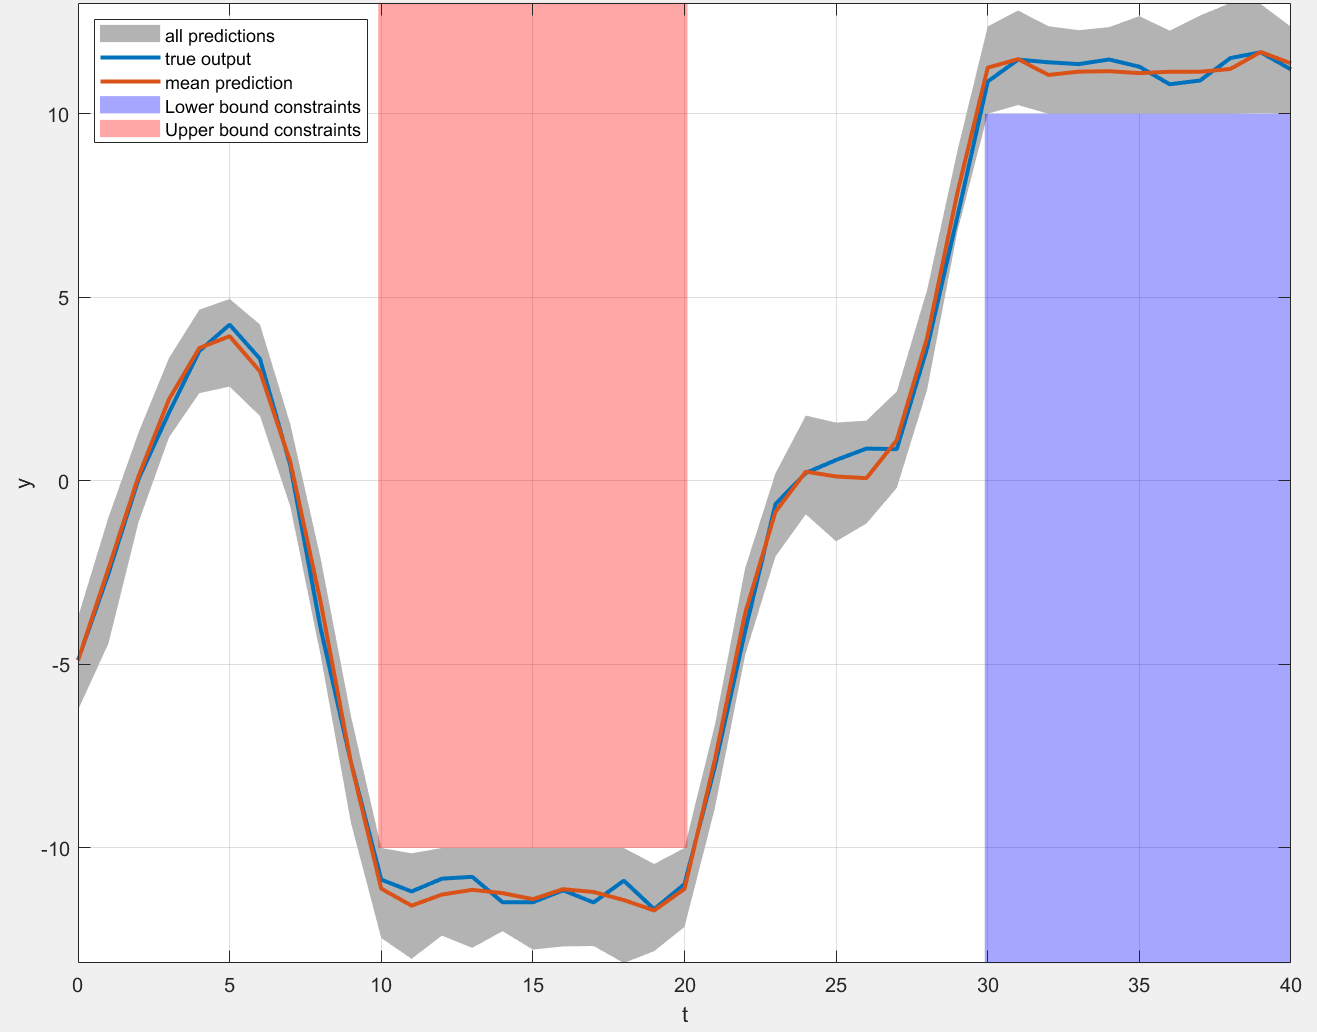
\includegraphics[width=0.4\textwidth] {pics/Scenario_plot.png}
   \label{fig:subfigScenario}
 }
\quad % puts next subfigure right next to the previous subfigure
\subfigure[Kernel Approach]{
   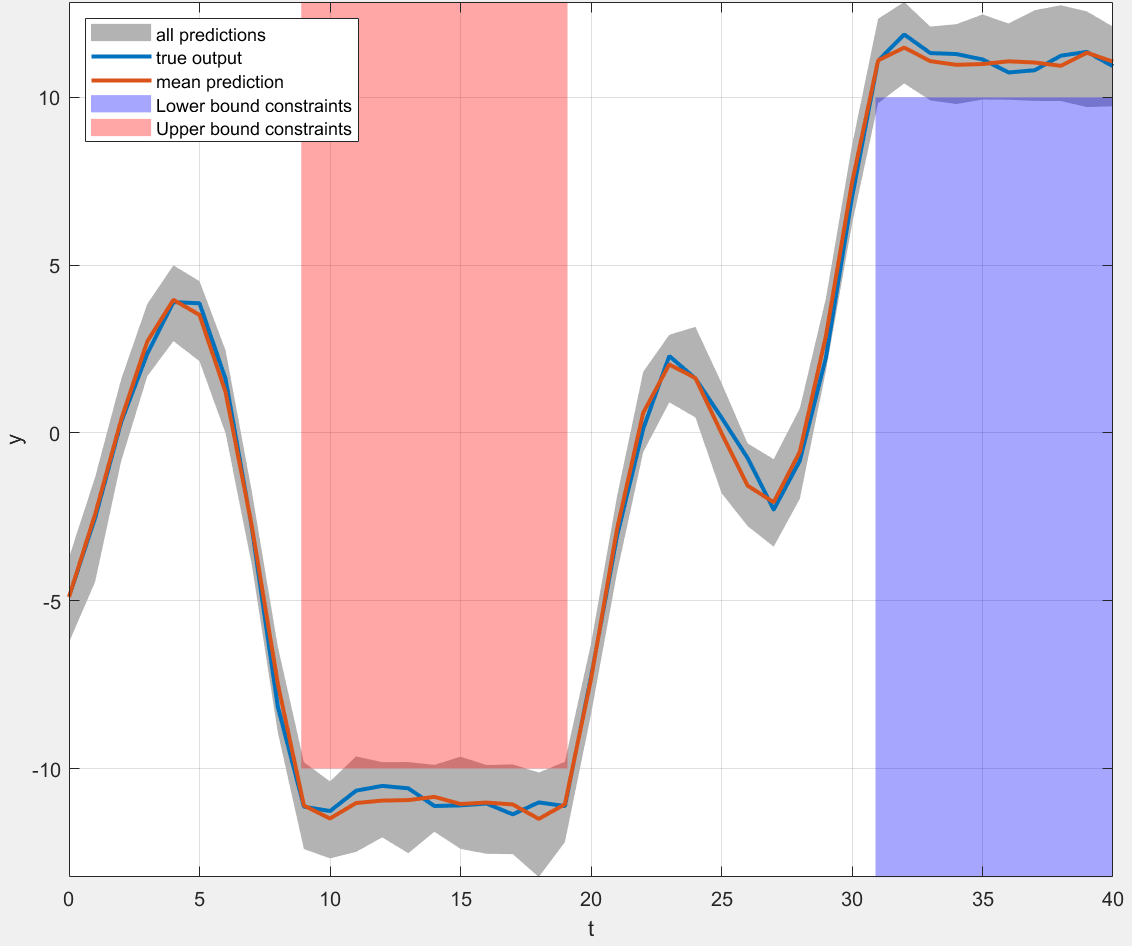
\includegraphics[width=0.4\textwidth] {pics/Kernel_plot.png}
   \label{fig:subfigKernel}
 }
\caption{Example of the optimal control with known basis functions for scenario approach (left) and kernel approach (right). The red and blue area show the output constraints. The gray area encompasses the 200 scenarios that were used in the optimization with the orange line being the average. The blue line is one realization of the true output.}
\label{ScenarioKernelComparison}
\end{figure}
\fi

\begin{figure}[htb]
\centering
\subfigure[Scenario Approach]{
\pgfplotsset{width=.47\textwidth, compat = 1.18, 
			height = .4\textwidth, grid= major, 
			legend cell align = left, ticklabel style = {font=\scriptsize},
			every axis label/.append style={font=\scriptsize},
			legend style = {font=\scriptsize},
        }
		\def\file{data/Scenario_K200_S2.txt}
		
		\centering
		\begin{tikzpicture}
		\begin{axis}[
		grid=none,
		xmin=0, xmax=40,
		ymin=-14, ymax=14,
		xtick={0, 10, 20, 30, 40},
		ytick={-10, -5, 0, 5, 10},
		ylabel=$y$, xlabel=$t$,
		set layers=standard,
		reverse legend,
		legend style={font=\scriptsize, at={(1,0)},anchor=south east, row sep=2pt},
		ylabel shift = -6 pt]
		
		\addplot[name path=A, forget plot, thick, opacity=0.2] table[x=t,y=y_opt_max]{\file};
		\addplot[name path=B, thick, opacity=0.2] table[x=t,y=y_opt_min]{\file};
		\tikzfillbetween[of=A and B]{opacity=0.2};
		\addlegendentry{$\left\{y_{0:H}^{[1:N]} \right\}$}
		
		\addplot[ultra thick,black!20!green] table[x=t,y=y_pred]{\file};
		\addlegendentry{$\frac{1}{N}\sum\limits_{n=1}^N y_{0:H}^{[n]}$}
		
		\addplot[ultra thick, blue] table[x=t,y=y_true]{\file};
		\addlegendentry{$y_{0:H}$}
		
		\draw [fill=red, fill opacity=0.2,red, opacity=0.2] (10,15) rectangle (20,-10); 
		\draw [fill=red, fill opacity=0.2,red, opacity=0.2] (30,10) rectangle (40,-15); 
		\end{axis}
		\end{tikzpicture}
 }
%\quad % puts next subfigure right next to the previous subfigure
\subfigure[Kernel Approach ($\alpha = 0.01$)]{
\pgfplotsset{width=.47\textwidth, compat = 1.18, 
			height = .4\textwidth, grid= major, 
			legend cell align = left, ticklabel style = {font=\scriptsize},
			every axis label/.append style={font=\scriptsize},
			legend style = {font=\scriptsize},
        }
		\def\file{data/Kernel_K200_Alpha001_S2.txt}
		
		\centering
		\begin{tikzpicture}
		\begin{axis}[
		grid=none,
		xmin=0, xmax=40,
		ymin=-14, ymax=14,
		xtick={0, 10, 20, 30, 40},
		ytick={-10, -5, 0, 5, 10},
		%ylabel=$y$, 
		xlabel=$t$,
		set layers=standard,
		reverse legend,
		legend style={font=\scriptsize, at={(1,0)},anchor=south east, row sep=2pt},
		ylabel shift = -6 pt]
		
		\addplot[name path=A, forget plot, thick, opacity=0.2] table[x=t,y=y_opt_max]{\file};
		\addplot[name path=B, thick, opacity=0.2] table[x=t,y=y_opt_min]{\file};
		\tikzfillbetween[of=A and B]{opacity=0.2};
		\addlegendentry{$\left\{y_{0:H}^{[1:N]} \right\}$}
		
		\addplot[ultra thick,black!20!green] table[x=t,y=y_pred]{\file};
		\addlegendentry{$\frac{1}{N}\sum\limits_{n=1}^N y_{0:H}^{[n]}$}
		
		\addplot[ultra thick, blue] table[x=t,y=y_true]{\file};
		\addlegendentry{$y_{0:H}$}
		
		\draw [fill=red, fill opacity=0.2,red, opacity=0.2] (10,15) rectangle (20,-10); 
		\draw [fill=red, fill opacity=0.2,red, opacity=0.2] (30,10) rectangle (40,-15); 
		\end{axis}
		\end{tikzpicture}
 } 

\subfigure[Kernel Approach ($\alpha = 0.2$)]{
\pgfplotsset{width=.47\textwidth, compat = 1.18, 
			height = .4\textwidth, grid= major, 
			legend cell align = left, ticklabel style = {font=\scriptsize},
			every axis label/.append style={font=\scriptsize},
			legend style = {font=\scriptsize},
        }
		\def\file{data/Kernel_K200_Alpha02_S2.txt}
		
		\centering
		\begin{tikzpicture}
		\begin{axis}[
		grid=none,
		xmin=0, xmax=40,
		ymin=-14, ymax=14,
		xtick={0, 10, 20, 30, 40},
		ytick={-10, -5, 0, 5, 10},
		ylabel=$y$, xlabel=$t$,
		set layers=standard,
		reverse legend,
		legend style={font=\scriptsize, at={(1,0)},anchor=south east, row sep=2pt},
		ylabel shift = -6 pt]
		
		\addplot[name path=A, forget plot, thick, opacity=0.2] table[x=t,y=y_opt_max]{\file};
		\addplot[name path=B, thick, opacity=0.2] table[x=t,y=y_opt_min]{\file};
		\tikzfillbetween[of=A and B]{opacity=0.2};
		\addlegendentry{$\left\{y_{0:H}^{[1:N]} \right\}$}
		
		\addplot[ultra thick,black!20!green] table[x=t,y=y_pred]{\file};
		\addlegendentry{$\frac{1}{N}\sum\limits_{n=1}^N y_{0:H}^{[n]}$}
		
		\addplot[ultra thick, blue] table[x=t,y=y_true]{\file};
		\addlegendentry{$y_{0:H}$}
		
		\draw [fill=red, fill opacity=0.2,red, opacity=0.2] (10,15) rectangle (20,-10); 
		\draw [fill=red, fill opacity=0.2,red, opacity=0.2] (30,10) rectangle (40,-15); 
		\end{axis}
		\end{tikzpicture}
 }
%\quad % puts next subfigure right next to the previous subfigure
\subfigure[Kernel Approach ($\alpha = 0.5$)]{
\pgfplotsset{width=.47\textwidth, compat = 1.18, 
			height = .4\textwidth, grid= major, 
			legend cell align = left, ticklabel style = {font=\scriptsize},
			every axis label/.append style={font=\scriptsize},
			legend style = {font=\scriptsize},
        }
		\def\file{data/Kernel_K200_Alpha05_S2.txt}
		
		\centering
		\begin{tikzpicture}
		\begin{axis}[
		grid=none,
		xmin=0, xmax=40,
		ymin=-14, ymax=14,
		xtick={0, 10, 20, 30, 40},
		ytick={-10, -5, 0, 5, 10},
		%ylabel=$y$, 
		xlabel=$t$,
		set layers=standard,
		reverse legend,
		legend style={font=\scriptsize, at={(1,0)},anchor=south east, row sep=2pt},
		ylabel shift = -6 pt]
		
		\addplot[name path=A, forget plot, thick, opacity=0.2] table[x=t,y=y_opt_max]{\file};
		\addplot[name path=B, thick, opacity=0.2] table[x=t,y=y_opt_min]{\file};
		\tikzfillbetween[of=A and B]{opacity=0.2};
		\addlegendentry{$\left\{y_{0:H}^{[1:N]} \right\}$}
		
		\addplot[ultra thick,black!20!green] table[x=t,y=y_pred]{\file};
		\addlegendentry{$\frac{1}{N}\sum\limits_{n=1}^N y_{0:H}^{[n]}$}
		
		\addplot[ultra thick, blue] table[x=t,y=y_true]{\file};
		\addlegendentry{$y_{0:H}$}
		
		\draw [fill=red, fill opacity=0.2,red, opacity=0.2] (10,15) rectangle (20,-10); 
		\draw [fill=red, fill opacity=0.2,red, opacity=0.2] (30,10) rectangle (40,-15); 
		\end{axis}
		\end{tikzpicture}
 } 


\caption{Example of the optimal control with known basis functions for scenario approach (top left) and kernel approach for various values of $\alpha$. The red areas show the output constraints. The gray area encompasses the 200 scenarios that were used in the optimization with the green line being the average. The blue line is one realization of the true output.}
\label{ScenarioKernelComparison}
\end{figure}



The figure includes the two plots for the scenario and kernel approach and shows the output $y$ of their respective OCPs. The graphs shows the spread of the $N = 200$ trajectories that are generated when the input $\boldsymbol{u}_{0:H}$ is applied to the scenarios that were used to find the optimal input. On top that, it also shows of the mean of these trajectories and true output. Where the two graphs differ however is to what extend the solutions fulfill the constraints. By its definition, the scenario approach requires all scenarios to fulfill the constraints which can be seen in the solution. While the gray area touches the lower and upper bounds during several timesteps, it never violates the constraints. The kernel approach on the other hand has a risk factor $\alpha$ built in which allows for a number of scenarios to violate the constraints as long a sufficient number satisfies them. This can be seen in the constraint still being met by the majority of the scenarios and only the trajectory of a small number of scenarios actively overlapping with the marked area. As a result, a solution with a lower cost was found in exchange for an increased risk of the true output violating one or more of the constraints.




\section{Robustness} \label{performance guarantees}

The biggest advantage that this kernel approximation proves compared to the scenario approach is the adjustable risk factor. As described in Sec. \ref{Sec:CCOKernel}, this method includes a parameter $\alpha \in [0, 1]$ which can be chosen depending on how successful the final solution is supposed to be when it comes to satisfying the constraints in future scenarios. 

In this section, this parameter is tested by running the same problem setup as was used in Sec. \ref{optimal control} for different values of $\alpha$ as well as increasing and lowering the number of samples $N$ and testing how well the solution holds up for other scenarios that are independent of the ones used in the optimization.

Similar to Sec. \ref{optimal control}, a number of scenarios are generated with Algorithm \ref{alg:PGibbs}. From this set of scenarios, a small subset is then taken and used to formulate several OCPs as was already described in Sec. \ref{optimal control}. The OCPs are then solved and the resulting optimal input $\boldsymbol{u}_{0:H}$ is applied to $N = 2000$ more independant scenarios from the same system to test how well this solution holds up. For each of the 2000 scenarios, the output is calculated and compared to the constraints that were used in the OCP to check whether or not they are fulfilled. This process is then repeated for various numbers of scenarios. It is done for 1, 5, 10 and 25 samples and then increased with a step size of 25 until $N = 250$ samples are used in the optimization.

\iffalse
\begin{figure}[htb]
\centering
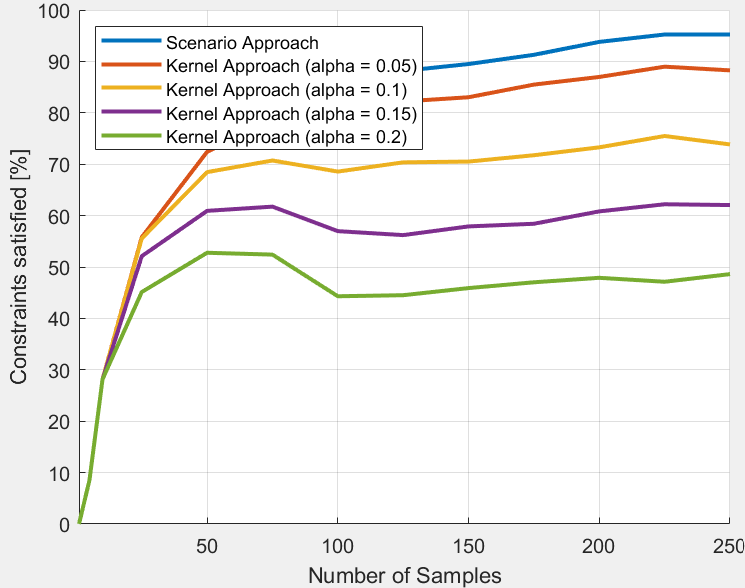
\includegraphics[width=0.7\textwidth]{pics/robustness_plot.png}
\caption{Percentage of scenarios where $u_{0:H}$ is a viable solution. The blue line shows the result of the scenario approach while the other lines are for the Kernel approach with various values of $\alpha$}
\label{fig:robustness_plot}
\end{figure}
\fi

\begin{figure}[t]
		\pgfplotsset{width=13cm, compat = 1.18, 
			height = 9cm, grid= major, 
			legend cell align = left, ticklabel style = {font=\scriptsize},
			every axis label/.append style={font=\scriptsize},
			legend style = {font=\scriptsize},
        }
		\def\file{data/AlphaTest_K200_MaxConstraint_S2.txt}
		
		\centering
		\begin{tikzpicture}
		\begin{axis}[
		grid=both,
		xmin=1, xmax=200,
		ymin=0, ymax=100,
		xtick={0, 50, 100, 150, 200, 250},
		ytick={0, 20, 40, 60, 80, 100},
		ylabel={Constraints Satisfied [\%]}, xlabel=$N$,
		set layers=standard,
		reverse legend,
		legend style={font=\scriptsize, at={(1,0)},anchor=south east, row sep=2pt},
		ylabel shift = -6 pt]
		
		\addplot[thick,black!20!red] table[x=K,y=Kernel04]{\file};
		\addlegendentry{Kernel Approach ($\alpha = 0.4$)}
		
		\addplot[thick,black!20!orange] table[x=K,y=Kernel03]{\file};
		\addlegendentry{Kernel Approach ($\alpha = 0.3$)}

		\addplot[thick,black!20!yellow] table[x=K,y=Kernel02]{\file};
		\addlegendentry{Kernel Approach ($\alpha = 0.2$)}

		\addplot[thick,black!20!green] table[x=K,y=Kernel01]{\file};
		\addlegendentry{Kernel Approach ($\alpha = 0.1$)}

		\addplot[thick,black!20!blue] table[x=K,y=Scenario]{\file};
		\addlegendentry{Scenario Approach}
		\end{axis}
		\end{tikzpicture}
		\vspace*{-0.4cm}
		
		\caption{Percentage of scenarios where $u_{0:H}$ is a viable solution. The blue line shows the result of the scenario approach while the other lines are for the kernel approach with various values of $\alpha$.}
		\label{fig:robustness_plot}
\end{figure}


In Fig. \ref{fig:robustness_plot} the results of this simulation are shown. The percentage of scenarios that fulfill the constraints is plotted over the number of samples used in the initial optimization which range from $N = 1$ to 250. The various $\alpha$ values are shown as separate lines. Initially, all five plots show very similar results. This can be explained by the fact that at such a low number of scenarios cannot accurately represent the distribution. As the number of scenarios is increased, the approximation of the distribution becomes better leading to a higher percentage of scenarios where the constraints are satisfied.

After around 10 scenarios, the plots start diverging for the first time. While the scenario approach and the plots with smaller $\alpha$ values are very similar, the lines that represent larger $\alpha$ values are starting to display worse percentage of cases that satisfy the constraints. This trend continues as the number of scenarios used in the optimization keeps increasing. While the scenario approach keeps increasing, the kernel approach seems to converge to a significantly lower level of robustness based on the selection of the parameter $\alpha$. This shows that through $\alpha$ we are able to control how distributionally robust the solution is.

As the number of scenarios used in the optimization keeps increasing, first signs of their behavior for $N \to \infty$ become visible. While we require more samples to be sure of the exact percentages the approaches are converging to, it is already clear that they are not converging towards $(1 - \alpha)$ as we has hoped. For example, the line for the kernel approach with $\alpha = 0.2$ does not converge to 80\% but instead a value around 50\%. It can also be shown that this percentage is highly dependent on the number and types of constraints used. That is because the way the constraints are set up does not lend itself to precisely controlling the ratio between cases that satisfy all of the constraints and cases that violate one or more of them. This can potentially be solved by replacing the $n_c$ constraints with a single one of the form $\text{max}(\boldsymbol{h}(\cdot)) \leq 0$ which will require further testing in the future.
 
\section{Corridor Test}

\begin{figure}[htb]
\centering
\subfigure[Scenario Approach]{
\pgfplotsset{width=.47\textwidth, compat = 1.18, 
			height = .4\textwidth, grid= major, 
			legend cell align = left, ticklabel style = {font=\scriptsize},
			every axis label/.append style={font=\scriptsize},
			legend style = {font=\scriptsize},
        }
		\def\file{data/Scenario_K100_N50.txt}
		
		\centering
		\begin{tikzpicture}
		\begin{axis}[
		grid=none,
		xmin=0, xmax=20,
		ymin=-12, ymax=4,
		xtick={0, 5, 10, 15, 20},
		ytick={-12, -8, -4, 0, 4},
		ylabel=$y$, xlabel=$t$,
		set layers=standard,
		reverse legend,
		legend style={font=\scriptsize, at={(1,0)},anchor=south east, row sep=2pt},
		ylabel shift = -6 pt]
		
		%\addplot[name path=A, forget plot, thick, opacity=0.2] table[x=t,y=y_opt_max]{\file};
		\foreach \index in {1,...,47}
			\addplot[thin, blue] table[x=t,y=Successful\index]{\file};
		%\addlegendentry{$y_{0:H}$}
		\foreach \index in {1,...,3}
			\addplot[thin, red] table[x=t,y=Failed\index]{\file};

		\draw [fill=red, fill opacity=0.2,red, opacity=0.2] (5,-5) -- (15,-5) arc(0:-180:5) --cycle;
		\draw [fill=red, fill opacity=0.2,red, opacity=0.2] (5,15) rectangle (15,-2.5); 
		%\draw [fill=red, fill opacity=0.2,red, opacity=0.2] (30,10) rectangle (40,-15); 
		\end{axis}
		\end{tikzpicture}
 }
\subfigure[Kernel Approach ($\alpha = 0.1$)]{
\pgfplotsset{width=.47\textwidth, compat = 1.18, 
			height = .4\textwidth, grid= major, 
			legend cell align = left, ticklabel style = {font=\scriptsize},
			every axis label/.append style={font=\scriptsize},
			legend style = {font=\scriptsize},
        }
		\def\file{data/Kernel_K100_N50_Alpha01.txt}
		
		\centering
		\begin{tikzpicture}
		\begin{axis}[
		grid=none,
		xmin=0, xmax=20,
		ymin=-12, ymax=4,
		xtick={0, 5, 10, 15, 20},
		ytick={-12, -8, -4, 0, 4},
		ylabel=$y$, xlabel=$t$,
		set layers=standard,
		reverse legend,
		legend style={font=\scriptsize, at={(1,0)},anchor=south east, row sep=2pt},
		ylabel shift = -6 pt]
		
		%\addplot[name path=A, forget plot, thick, opacity=0.2] table[x=t,y=y_opt_max]{\file};
		\foreach \index in {1,...,47}
			\addplot[thin, blue] table[x=t,y=Successful\index]{\file};
		%\addlegendentry{$y_{0:H}$}
		\foreach \index in {1,...,3}
			\addplot[thin, red] table[x=t,y=Failed\index]{\file};

		\draw [fill=red, fill opacity=0.2,red, opacity=0.2] (5,-5) -- (15,-5) arc(0:-180:5) --cycle;
		\draw [fill=red, fill opacity=0.2,red, opacity=0.2] (5,15) rectangle (15,-2.5); 
		%\draw [fill=red, fill opacity=0.2,red, opacity=0.2] (30,10) rectangle (40,-15); 
		\end{axis}
		\end{tikzpicture}
 }
\subfigure[Kernel Approach ($\alpha = 0.2$)]{
\pgfplotsset{width=.47\textwidth, compat = 1.18, 
			height = .4\textwidth, grid= major, 
			legend cell align = left, ticklabel style = {font=\scriptsize},
			every axis label/.append style={font=\scriptsize},
			legend style = {font=\scriptsize},
        }
		\def\file{data/Kernel_K100_N50_Alpha02.txt}
		
		\centering
		\begin{tikzpicture}
		\begin{axis}[
		grid=none,
		xmin=0, xmax=20,
		ymin=-12, ymax=4,
		xtick={0, 5, 10, 15, 20},
		ytick={-12, -8, -4, 0, 4},
		ylabel=$y$, xlabel=$t$,
		set layers=standard,
		reverse legend,
		legend style={font=\scriptsize, at={(1,0)},anchor=south east, row sep=2pt},
		ylabel shift = -6 pt]
		
		%\addplot[name path=A, forget plot, thick, opacity=0.2] table[x=t,y=y_opt_max]{\file};
		\foreach \index in {1,...,48}
			\addplot[thin, blue] table[x=t,y=Successful\index]{\file};
		%\addlegendentry{$y_{0:H}$}
		\foreach \index in {1,...,2}
			\addplot[thin, red] table[x=t,y=Failed\index]{\file};

		\draw [fill=red, fill opacity=0.2,red, opacity=0.2] (5,-5) -- (15,-5) arc(0:-180:5) --cycle;
		\draw [fill=red, fill opacity=0.2,red, opacity=0.2] (5,15) rectangle (15,-2.5); 
		%\draw [fill=red, fill opacity=0.2,red, opacity=0.2] (30,10) rectangle (40,-15); 
		\end{axis}
		\end{tikzpicture}
 }
%\quad % puts next subfigure right next to the previous subfigure
\subfigure[Kernel Approach ($\alpha = 0.3$)]{
\pgfplotsset{width=.47\textwidth, compat = 1.18, 
			height = .4\textwidth, grid= major, 
			legend cell align = left, ticklabel style = {font=\scriptsize},
			every axis label/.append style={font=\scriptsize},
			legend style = {font=\scriptsize},
        }
		\def\file{data/Kernel_K100_N50_Alpha03.txt}
		
		\centering
		\begin{tikzpicture}
		\begin{axis}[
		grid=none,
		xmin=0, xmax=20,
		ymin=-12, ymax=4,
		xtick={0, 5, 10, 15, 20},
		ytick={-12, -8, -4, 0, 4},
		ylabel=$y$, xlabel=$t$,
		set layers=standard,
		reverse legend,
		legend style={font=\scriptsize, at={(1,0)},anchor=south east, row sep=2pt},
		ylabel shift = -6 pt]
		
		%\addplot[name path=A, forget plot, thick, opacity=0.2] table[x=t,y=y_opt_max]{\file};
		\foreach \index in {1,...,47}
			\addplot[thin, blue] table[x=t,y=Successful\index]{\file};
		%\addlegendentry{$y_{0:H}$}
		\foreach \index in {1,...,3}
			\addplot[thin, red] table[x=t,y=Failed\index]{\file};

		\draw [fill=red, fill opacity=0.2,red, opacity=0.2] (5,-5) -- (15,-5) arc(0:-180:5) --cycle;
		\draw [fill=red, fill opacity=0.2,red, opacity=0.2] (5,15) rectangle (15,-2.5); 
		%\draw [fill=red, fill opacity=0.2,red, opacity=0.2] (30,10) rectangle (40,-15); 
		\end{axis}
		\end{tikzpicture}
 }
\caption{Example of the optimal control with known basis functions for scenario approach (top left) and kernel approach. The red areas show the output constraints. The lines show trajectories of the true system. The outputs that successfully avoid the constraints are colored blue, while all the outputs that violate at least one constraint are colored red.}

\label{ScenarioKernelComparisonCorridor}
\end{figure}
